\documentclass[11pt]{ctexart}
\usepackage{amsmath,amssymb}
\usepackage[margin=1in]{geometry}
\usepackage{booktabs}
\usepackage{enumitem}
\usepackage{graphicx}
\usepackage{float}

\begin{document}

\title{线性回归分析 第6周作业实验报告}
\author{}
\date{}
\maketitle

\section*{Problem 3.7（KNNL3.7）：残差诊断}

残差定义为
\[
e_i=Y_i-\hat Y_i.
\]

\subsection*{3.7(a) 年龄 \(X_i\) 的茎叶图}

年龄的茎叶图如下（茎为十位数，叶为个位数）：
\begin{verbatim}
4 | 111223345677788
5 | 12334456777999
6 | 000133345556889
7 | 0012235666788888
\end{verbatim}

四个十年组的叶数约为 \(15,14,15,16\)。四个年龄组均有较充分的观测，且各十年组内年龄分布较分散。总体上这与“从每个 10 岁年龄组随机抽取 15 名妇女”的分层抽样设计基本一致；个别边界年龄的归组会造成各茎叶数的轻微差异，但不显示明显的系统性缺口。

\subsection*{3.7(b) 残差及残差直方图}

全部 60 个残差满足
\[
\sum_{i=1}^{60} e_i\approx 0,\qquad
\min e_i=-16.1366,\qquad
\max e_i=23.4734.
\]
残差直方图见图 \ref{fig:hist}。直方图大致以 0 为中心，主体近似对称；但存在一个较大的正残差 \(e_{53}=23.4734\)（对应 \(X=78\)），说明该观测的肌肉质量明显高于线性回归拟合值。

\begin{figure}[H]
\centering
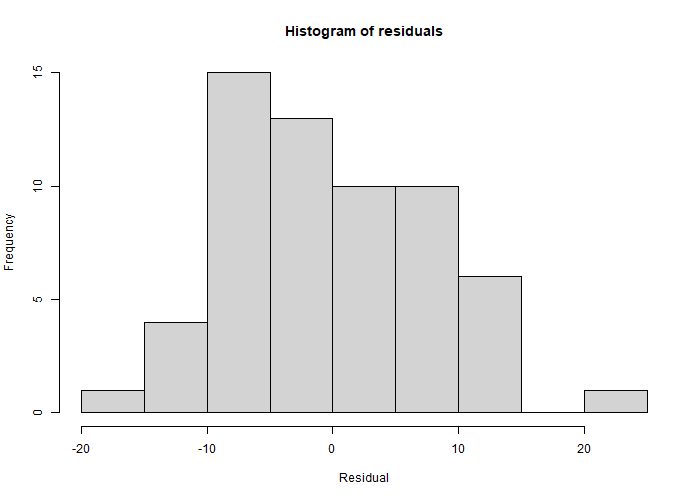
\includegraphics[width=0.75\linewidth]{p1b_hist.png}
\caption{残差直方图}
\label{fig:hist}
\end{figure}

\subsection*{3.7(c) 残差对 \(\hat Y_i\) 与对 \(X_i\) 的图}

残差对拟合值 \(\hat Y_i\) 的图见图 \ref{fig:resfit}，残差对 \(X_i\) 的图见图 \ref{fig:resx}。

\begin{figure}[H]
\centering
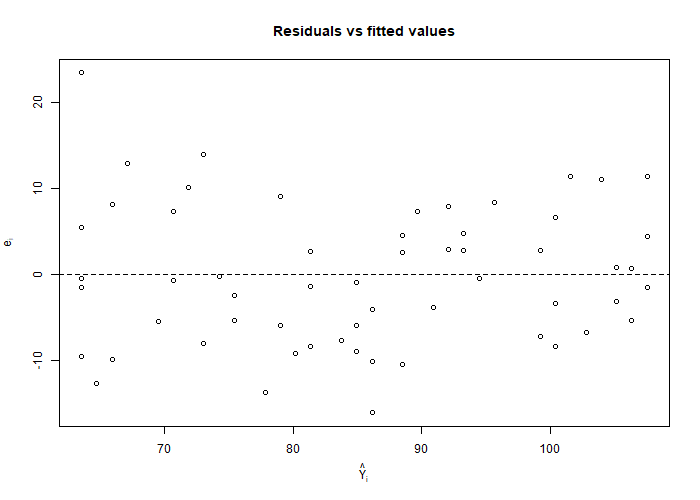
\includegraphics[width=0.75\linewidth]{p1c_fitted.png}
\caption{残差 \(e_i\) 对拟合值 \(\hat Y_i\)}
\label{fig:resfit}
\end{figure}

\begin{figure}[H]
\centering
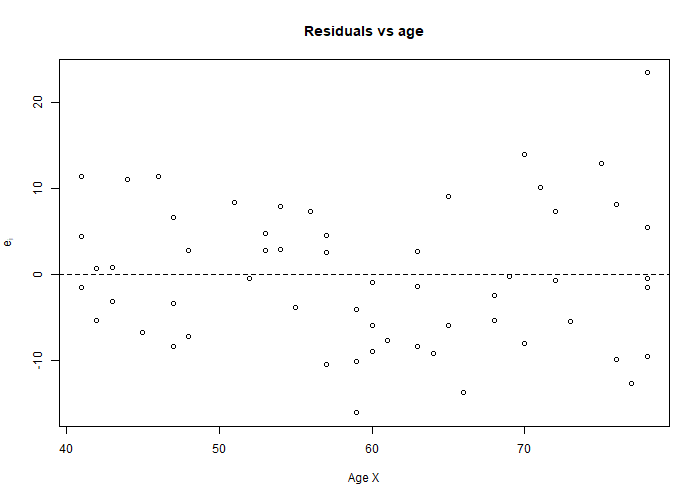
\includegraphics[width=0.75\linewidth]{p1c_x.png}
\caption{残差 \(e_i\) 对年龄 \(X_i\)}
\label{fig:resx}
\end{figure}

两图均未显示明显的曲线趋势，说明一阶线性模型基本合适。由于
\[
\hat Y_i=156.3466-1.1900X_i
\]
是 \(X_i\) 的严格线性函数，因此残差对 \(\hat Y_i\) 与残差对 \(X_i\) 的图形本质上提供相同信息，只是横轴经过线性变换且方向相反。图中可见高龄组（尤其 \(X=78\)）残差离散程度略大，并有一个很大的正残差，但尚无非常强烈的异方差“漏斗形”证据。

\subsection*{3.7(d) 残差正态概率图与正态性相关系数}

正态概率图见图 \ref{fig:qq}。取期望正态分数
\[
z_i=\Phi^{-1}\left(\frac{i-3/8}{n+1/4}\right),\qquad n=60,
\]
计算有序残差 \(e_{(i)}\) 与 \(z_i\) 的相关系数，得
\[
r_Q=\operatorname{corr}\bigl(e_{(i)},z_i\bigr)\approx 0.9896.
\]
查表 B.6，取 \(\alpha=0.10\)、\(n=60\)，临界值约为
\[
r^*_{0.10,60}\approx 0.978.
\]
因为
\[
r_Q=0.9896>r^*_{0.10,60}\approx 0.978,
\]
所以不拒绝正态性假定。正态概率图总体接近直线，仅右尾受一个较大正残差影响略有偏离；在 \(\alpha=0.10\) 下仍可认为误差正态性假定合理。

\begin{figure}[H]
\centering
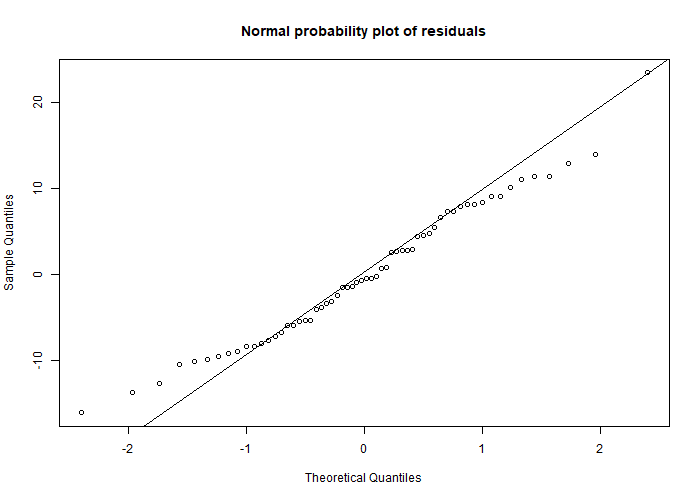
\includegraphics[width=0.75\linewidth]{p1d_qq.png}
\caption{残差正态概率图}
\label{fig:qq}
\end{figure}

\subsection*{3.7(e) Breusch-Pagan 检验}

检验误差方差是否随 \(X\) 变化。令
\[
u_i=\frac{e_i^2}{\hat\sigma^2},\qquad \hat\sigma^2=MSE=66.8008.
\]
对 \(u_i\) 关于 \(X_i\) 作辅助回归，得
\[
\hat u_i=-0.768+0.02947X_i,
\]
辅助回归的回归平方和为
\[
SSR^*=7.133.
\]
Breusch-Pagan 统计量为
\[
X_{BP}^2=\frac{SSR^*}{2}=\frac{7.133}{2}=3.57.
\]

检验假设为
\[
H_0:\ \sigma_i^2=\sigma^2\ \text{（误差方差为常数）},
\]
\[
H_1:\ \sigma_i^2\ \text{随 }X_i\text{ 变化}.
\]
取 \(\alpha=0.01\)，自由度为 1 的卡方临界值为
\[
\chi^2_{0.99,1}=6.6349.
\]
决策规则：若 \(X_{BP}^2>\chi^2_{0.99,1}\)，拒绝 \(H_0\)。

由于
\[
X_{BP}^2=3.57<6.6349,
\]
故不拒绝 \(H_0\)。在 \(\alpha=0.01\) 下，没有充分证据认为误差方差随年龄 \(X\) 变化。该结论与 3.7(c) 中残差图未出现明显异方差趋势的初步判断一致；尽管高龄组有一个较大残差，但 Breusch-Pagan 检验在 \(1\%\) 水平下不显著（近似 \(p\approx 0.059\)）。

\section*{Prob2}
乍一看是个废话，实际上是指工资的中位数低于平均值，反映出它是right-skewed的。也就是说，工资分布中有一些高收入者拉高了平均值，而大多数人的工资低于平均值，因此中位数低于平均值。
但写在报纸标题就很诡异。

\end{document}